\documentclass{standalone}
% preamble: usepackage, etc.
\begin{document}

\chapter{latex设置说明}

(注意段落标题之间不能有空白必须有正文)(注意段落标题之间不能有空白必须有正文)(注意段落标题之间不能有空白必须有正文)(注意段落标题之间不能有空白必须有正文)(注意段落标题之间不能有空白必须有正文)

\label{chap2}

\section{语言模式}

本模板只有一套中文基础语言环境。改变语言环境会改变图表标题的引导词(图,表),文章结构词(比如目录,参考文献等),以及定理环境中的引导词(比如定理,引理等)。段落等文字直接粘贴即可,格式均自动调整。

\section{标题设置}
以下为各级标题格式:

1) {chapter}为一级标题提示符;

2)  {section}为二级标题提示符;

3)  {subsection}为三级标题提示符。

\section{图片设置}
{figure}为插入图片提示符,本latex所使用的图片应为矢量图格式,即.pdf格式。
由于插入的图片为.png或.jpg时可能会出现图片不清晰,缩放会失真,将图片转换为矢量图可编辑性更好,更适合印刷。

\subsection{图片格式转换}

尽量使用微软visio和Adobe AI等软件制作矢量图,新版模版论文支持矢量图,打印和放缩都会清晰不失真。如果不会只用JPG,可以将.jpg或者.png文件转换为.pdf格式的详细方法:

1)将.jpg或者.png文件上传到\href{https://img.logosc.cn/?utm_source=zhihutg05.com/}{https://texstudio.sourceforge.net/},点击AI改图——文件格式转换,选择转换方式为pdf,点击下载完成;

2)如果失效,请点击:\href{https://www.zhihu.com/question/292896684}{https://texstudio.sourceforge.net/}。


\subsection{图片引用}
label为图片引用标签,如图\ref{fig_20}所示。
\begin{figure}[htbp]
	\centering
	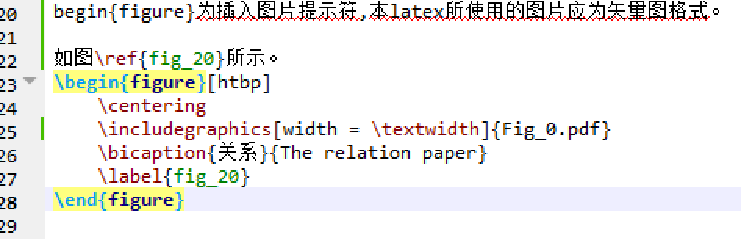
\includegraphics[width = \textwidth]{a11.pdf}
	\bicaption{图片引用方式}{Image reference mode}
	\label{fig_20}
\end{figure}



\section{公式引用}\label{sec_face_landmark}
 
 文中所有外文计量单位(如千克kg)、固定标准函数(如三角函数)、事物名称、数字、数学运算符等用正体,外文变量或物理量、非固定标准函数都用斜体,向量、集合、矩阵、张量用粗斜体(上下标不用加粗)。

语言的使用过程是人们在受语言内部或者外部因素的驱动下有意无意不断进行语言选择的过程$E_1, E_2, \dots,E_n, \dots, E_{N_E}$和一个门控神经网络$G$所组成的。

\begin{equation}
	a = - \sum_{i=1}^{n}{y_i\:\log(\hat{y_i})} +     \label{eq:0}
	\lambda {\left\lVert\omega\right\rVert}_2^2
\end{equation}


\begin{equation}\label{eq_fs_parameter}
	b_{j} = \left\{\begin{array}{lcl}
		f_{j} & \text{if} & k=1\\ 
		f_{i} & \text{if} & k=N_{fs}
	\end{array}\right.
\end{equation}


商讨性和顺应性三个相互关联的本质属性。因此,式(\ref{eq_fs_parameter})为所引用公式,两者名称应一致,如图\ref{fig_11}。

\begin{figure}[htbp]
	\centering
	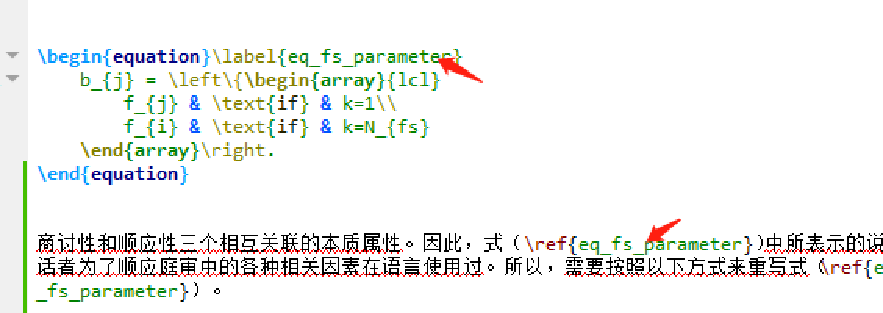
\includegraphics[width = \textwidth]{a12.pdf}
	\bicaption{公式引用}{The relation paper}
	\label{fig_11}
\end{figure}

更多相关公式的例子请参考:\href{https://zhuanlan.zhihu.com/p/110756681}{https://zhuanlan.zhihu.com/p/110756681}


\end{document}
